% Use the following line  only  if you're still using LaTeX 2.09.
%\documentstyle[icml2014,epsf,natbib]{article}
% If you rely on Latex2e packages, like most moden people use this:
\documentclass{article}
% use Times
\usepackage{times}
 % For figures
\usepackage{graphicx} % more modern
%\usepackage{epsfig} % less modern
\usepackage{subfigure} 
\usepackage{footnote}
\usepackage{amsfonts}
\usepackage{mdframed}

% For citations
\usepackage{natbib}
\usepackage{comment}
\usepackage{multirow}

\usepackage{float}

\floatstyle{plain} % optionally change the style of the new float
\newfloat{code}{H}{myc}

% For algorithms
\usepackage{algorithm}
\usepackage{algorithmic}
\usepackage{amsmath}
\usepackage{listings}

\lstset{language=Python,
  basicstyle=\ttfamily\footnotesize,
  keywordstyle=\color{blue}\ttfamily,
  stringstyle=\color{red}\ttfamily,
  commentstyle=\color{green}\ttfamily,
  aboveskip=0pt,
  belowskip=0pt,
  breaklines=true
}

\setlength{\abovedisplayskip}{0cm}
\setlength{\belowdisplayskip}{0cm}

\usepackage{mathtools}


\newcommand\myeq{\stackrel{\mathclap{\normalfont\mbox{{\tiny def}}}}{=}}


\usepackage[compact]{titlesec}
\titlespacing{\section}{0pt}{0.5ex}{0.3ex}
\titlespacing{\subsection}{0pt}{0.2ex}{0ex}
\titlespacing{\subsubsection}{0pt}{0.1ex}{0ex}

\newcommand{\startcompact}[1]{\par\vspace{-0.75em}\begin{#1}%
  \allowdisplaybreaks\ignorespaces}

\newcommand{\stopcompact}[1]{\end{#1}\ignorespaces}

\usepackage{paralist}

\makeatletter
\ifcase \@ptsize \relax% 10pt
  \newcommand{\miniscule}{\@setfontsize\miniscule{4}{5}}% \tiny: 5/6
\or% 11pt
  \newcommand{\miniscule}{\@setfontsize\miniscule{5}{6}}% \tiny: 6/7
\or% 12pt
  \newcommand{\miniscule}{\@setfontsize\miniscule{5}{6}}% \tiny: 6/7
\fi
\makeatother

\newcommand {\aplt} {\ {\raise-.5ex\hbox{$\buildrel<\over\sim$}}\ }

\newcommand{\eqn}[1]{Eqn.~\ref{eqn:#1}}
\newcommand{\fig}[1]{Fig.~\ref{fig:#1}}
\newcommand{\tab}[1]{Table~\ref{tab:#1}}
\newcommand{\secc}[1]{Section~\ref{sec:#1}}
\def\etal{{\textit{et~al.~}}}
\newcommand{\BigO}[1]{\ensuremath{\operatorname{O}\left(#1\right)}}
\usepackage[symbol*]{footmisc}

\DefineFNsymbolsTM{myfnsymbols}{% def. from footmisc.sty "bringhurst" symbols
  \textasteriskcentered *
  \textdagger    \dagger
  \textdaggerdbl \ddagger
  \textsection   \mathsection
  \textbardbl    \|%
  \textparagraph \mathparagraph
}%


% As of 2011, we use the hyperref package to produce hyperlinks in the
% resulting PDF.  If this breaks your system, please commend out the
% following usepackage line and replace \usepackage{icml2014} with
% \usepackage[nohyperref]{icml2014} above.
\usepackage{hyperref}

% Packages hyperref and algorithmic misbehave sometimes.  We can fix
% this with the following command.
\newcommand{\theHalgorithm}{\arabic{algorithm}}

% Employ the following version of the ``usepackage'' statement for
% submitting the draft version of the paper for review.  This will set
% the note in the first column to ``Under review.  Do not distribute.''
%\usepackage{icml2014} 
% Employ this version of the ``usepackage'' statement after the paper has
% been accepted, when creating the final version.  This will set the
% note in the first column to ``Proceedings of the...''
\usepackage[accepted]{icml2014}



\begin{document} 

\twocolumn[
\icmltitle{Learning to Reason\\{\small PhD Thesis Proposal}}

\icmlauthor{Wojciech Zaremba}{woj.zaremba@gmail.com}
\vskip +0.1in
\icmlauthor{Advisors:}{}
\vskip +0.03in
\icmlauthor{Rob Fergus}{fergus@cs.nyu.edu}
\vskip +0.03in
\icmlauthor{Yann LeCun}{yann@cs.nyu.edu}
\icmladdress{New York University}

\icmlkeywords{computer vision, convolutional neural networks, recursive neural networks, natural language processing, recurrent neural networks, language model, LSTMs, program understanding, artificial intelligence}

\vskip 0.3in
]

\begin{abstract}

  Neural networks have proven to be very powerful models for object
  recognition \cite{krizhevsky2012imagenet}, natural language
  processing \cite{mikolov2012statistical}, speech recognition
  \cite{graves2013speech}, and other tasks
  \cite{sutskever2014sequence}.  However, there is still a huge gap
  between them and a truly intelligent system.  I identify several
  qualities that an intelligent systems should possess, namely: (i)
  reasoning ability, (ii) the capability to integrate with external
  interfaces and (iii) small sample complexity. My thesis will focus on
  tackling these problems.

\end{abstract} 

\section{Introduction}
It is clear that improving the performance of current statistical learning systems, 
will not make them intelligent, even if they achieve
$0\%$ test error. This proposal explores what skills are necessary for statistical
learning system to become ``intelligent'' and outlines attempts to
provide these skills. 

While many qualities make up true intelligence, we focus on three
skills that are notably lacking from current approaches: (i) the
ability to reason, (ii) the capability to integrate with external
interfaces and (iii) small sample complexity. The goal is to provide
all of these skills within a single unified framework. This will be
approached via a wide range of tasks in different domains, to empirically
verify its robustness. 

For some of these tasks, exploratory work has already been performed 
giving good intuitions for the proposed work. 

\section{Reasoning abilities}

Reasoning is the process of forming conclusions, judgements, or
inferences from facts or premises. An artificial system that can
reason should be able to understand high level concepts like: 
\begin{itemize}
 \item Scope
 \item Conditioning
 \item Nesting
 \item Repetitions
 \item Memorization 
 \end{itemize}
While each of this skills could be solved in a particular domain; the
resulting system would be of little use and would require
strong assumptions about possible scenarios. Moreover, an intelligent
reasoning system cannot be based only on predefined rules. Instead, it
should be based on pattern matching, and the application of learned heuristic algorithms. 

There are many domains where we can test the reasoning ability of our
system to see if it is able to learn postulated concepts. These
include (a) computer programs and (b) the derivation of mathematical
theorems. Both of these are rich in scoping, branching, nesting,
pattern repetition, and so on. Drawing high-level conclusions in such
domains requires sophisticated reasoning. Eventually, the framework
should be able to handle many different domains simultaneously.

\subsection{Reasoning in computer programs}
The first reasoning task that I intend to tackle is to train
statistical models the meaning of computer programs.
Consider one possible instantiation of this, where the task is to take
a program as an input (e.g.~character-by-character), and predict the
program output. This requires the statistical model to understand
every single operand of a program. For instance, in the case of
addition it involves bit shifts, and memorization of operations on
digits. Moreover, programs can contain variable assignment, if-statements, and so on.
We were able partially to address this problem \cite{zaremba2014execute}.
Figure \ref{fig:prog} shows an exemplary program and its output, along
with a prediction of the output obtained with a recurrent neural network.

\begin{figure}
  \begin{code}
  \begin{mdframed}
  {\bf Input:}
  \begin{lstlisting}
  f=(8794 if 8887<9713 else (3*8334))
  print((f+574))
  \end{lstlisting} 
  {\bf Target:} 9368. \\
  {\bf Model prediction:} 9368. 
  \end{mdframed}
  \end{code}
  \caption{An example program that we take as an input. The task is
    to predict the evaluation of the program. We have 
  achieved a high level of performance on this task \cite{zaremba2014execute}.}
  \label{fig:prog}
\end{figure}


Although current results are promising, they are very limited. We are able to deal with programs
that can be evaluated by reading them once from left-to-right, but
generic programs are far more complex. Our reasoning system has to be
able to evaluate for an arbitrarily long time, if the
task requires it. Moreover, it shouldn't be limited by a fixed memory
size. Instead, memory should be available
as an interface (see Section \ref{sec:interface}).


\subsection{Reasoning in mathematics}
It is known that theorem proving is an intractable task in a computational sense. 
However, humans are able to prove theorems. They do this by employing prior
knowledge, acquired from experience of solving other, related
problems, and fitting known mathematical ``tricks'' to the new problem.

More formally, we can think about proofs as an application with
multiple axioms that starts with a 
hypothesis that we want to prove. Thus mathematical skills can be perceived as 
a learning prior over trees of axioms. This prior ``suggests'' which sequence of axioms is more
likely to lead to a proof of the theorem. 


My interest lies in training statistical machine learning systems to learn such priors. 
We have started with the very constrained mathematical domain of
polynomials and demonstrate that here we can learn a prior over mathematical identities. 
Our recent work \cite{zaremba2014learning} concerns identities 
over polynomials over matrices. Figure \ref{fig:ident} shows example of a simple identity
over matrix polynomials. It states that, $\sum_{i,j} \sum_k A_{i, k}B_{k, j} = 
\sum_{j} \sum_k (\sum_i A_{i, k})B_{k, j})$. This is an example of a toy identity. Our system is able
to derive much more sophisticated identities.


\begin{figure}
  \centering
  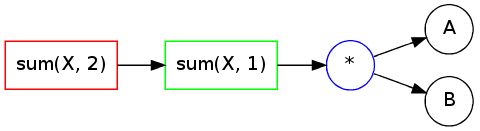
\includegraphics[width=0.48\textwidth]{imgs/example1_brute.png}\\
  {\bf Is equivalent to:}\\
  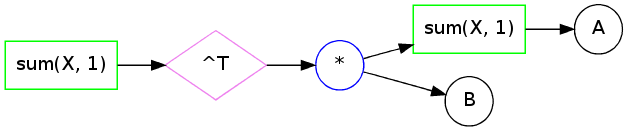
\includegraphics[width=0.48\textwidth]{imgs/example1_opt.png}\\
  \caption{An example of two equivalent mathematical expressions. It states that
  $\sum_{i,j} \sum_k A_{i, k}B_{k, j} = \sum_{j} \sum_k (\sum_i A_{i,
    k})B_{k, j})$. \cite{zaremba2014learning} contains much more sophisticated examples.}
  \label{fig:ident}
\end{figure}


\section{Interface learning}
\label{sec:interface}
Neural networks are very powerful statistical models, however some
concepts appears to be very difficult for them to express.  For instance,
nesting seems to be a very common operation, that allows one to deal
with (1) object hierarchies, (2) natural language parsing, and (3)
compositionality. I think that, the ability to nest concepts could be provided by
adding a stack as an external interface to the neural network, with
the neural network learning how to use such an interface.

More broadly, external interfaces could enhance neural networks capabilities, and also provide
access to external resources and datasets. Potentially useful
interfaces include:
\begin{itemize}
  \item stack
  \item FIFO
  \item external memory \cite{weston2014memory, graves2014neural}
  \item search engine
  \item database
  \item execution environment such as a python interpreter
\end{itemize}

The state space of many interfaces is massive (e.g.\ all possible search queries).
Moreover, external interfaces are non-differentiable.
These obstacles could potentially be addressed by learning a differentiable 
model that describes them (e.g.~a neural network). This network would simulate the
external interface for the purpose of being differentiable. 

\section{Small sample complexity}
Current deep learning systems suffer from large sample
complexity. This hinders the potential use of these systems for online 
learning (e.g.~robots). It is expected that during the initial phase of 
learning any system without prior knowledge would need to consume a large number of samples. 
However, we hope that as training progresses, sample complexity would drop. But this is 
not observed in current systems. I propose several approaches that would
allow sample complexity to be decreased. 
The meta-optimizer (see Subsection \ref{subsec:meta}) is the desired
solution, but I also propose some intermediate solutions that can also
decrease sample complexity.

\subsection{Automatic derivation of better models}
Neural networks are designed in an ad-hoc fashion, using a researcher's
intuition about what architectures will result in a high-prediction
performance. One way of addressing this issue would be to
fully understand why, and how the models work. However, mathematical
analyses give little insight and it is unclear if it is even 
possible. I would like to automatically
explore a large space of models, and evaluate them on various tasks. 
This involves trying different connectivity patterns, activation
functions, and hyper-parameter settings. To search over this discrete
space, I intend to use genetic programming. 


\subsection{Augmentation marginalization}
For simplicity, we focus on computer vision tasks.

We often train neural networks for multiple epochs, while the same 
samples are presented multiple times. The best performance is
achieved when samples are slightly modified over the course of training.
In case of computer vision, it is done by jittering images, rotating
them, and so on. This is known as data-augmentation. 
Theoretically, a full image contains information about all updates obtained
with all possible augmented samples. More formally, let $x$ be an image, $y$ its label, and
$x_1, x_2 \dots x_k$ are its augmented copies. $L$ is a loss function, and $\theta_i$ are parameters at step $i$. So $\theta_1$ is a initial set of parameters, and $\theta_{k+1}$ is a set of parameters after $k$ updates. 
I would like to
predict for a given $x$, the sum of the derivatives for all data augmentations:
\begin{align}
  f(x, \theta_1) = \sum_{i=1}^k \partial_\theta L(x_k, y, \theta_i) = \theta_{k+1} - \theta_1
\end{align}

Instead of following gradient of $\partial_\theta L(x, y, \theta_1)$, we could
follow $f(x, \theta_1)$.
This could improve learning speed, as a single sample would provide
information about all its augmented copies. 

The function $f$ might have its own parameters, and I would like to model it 
as a neural network which would be trained in a supervised fashion. 

\subsection{One-shot learning objective}
Human are able to recognize new objects after seeing them just once.
Contemporary deep learning systems are far from being able to do this,
requiring hundreds or even thousands of examples.  We propose a new
formulation of neural network training that focuses on training for the
one-shot learning objective.

The main idea is to train one neural network to predict parameters of another neural network. 
More formally, let $\phi(x, W_{in}, \theta) = (y, W_{y})$ be a neural network parametrized
by $\theta$. Weights $W_{in} \in \mathbb{R}^{f \times l}$ are top layer weights, where
$f$ is the top layer feature size, and $l$ is the number of labels. $W_{y} \in \mathbb{R}^f$ is a
single weight vector used to predict class $y$.

For a given new class $x', y'$, we compute $ W_{y'} = \phi(x', None, \theta)$ to produce weights $W_{y'}$. 
We use these weights to classify
other objects belonging to the class $y'$.
This idea is currently being explored with my collaborators Elias Bingham and Brenden Lake.

\subsection{Meta-optimizer}
\label{subsec:meta}
I would like to build a meta-optimizer that would be used to train a
neural network.  Such an optimizer would take as input the gradients
of a neural network, and would decide on the next update step. The
optimizer itself could be parameterized with another neural network,
which would allow it to simulate any first order, gradient-based,
learning algorithm like SGD, momentum, LBFGs etc. This implies that
such a meta-optimizer should subsume all first order, gradient-based
optimization techniques.  This work is under progress, 
supervised by my collaborator Rahul Krishnan and Anna Choromanska.

\section{Discussion}
Tackling the aforementioned problems would take us much closer to
real intelligent systems, and defines three core pillars 
of Artificial Intelligence. However, there are many other problems which 
need to be solved and integrated to achieve a fully 
intelligent system, e.g. navigation, learning by imitation, cooperation, and many others.

%However, I think that all that skills can be integrated by means of external interface, and
%don't have to be modeled in any special way. For instance, navigation skill could emerge 
%as an use two interfaces (1) GPS location interface, and (2) an external memory.


%\section{Disclaimer}
%This is my personal opinion, and it shouldn't be judged in a scientific way.


%I strongly believe that creation of artificial intelligence is potentially
%dangerous. However, I think, that more dangerous is avoiding to create it.
%We exhaust resources of our planet in rapid fashion, and lack of resources 
%leads to wars. The only way to prevent it is to have abundance of resources.
%Artificial intelligence could provide abundance of all resources.


\bibliography{bibliography}
\bibliographystyle{icml2014}

\end{document} 

